\documentclass[aspectratio=169]{beamer}

% Theme and Color Scheme
\usetheme{Madrid}
\usecolortheme{beaver}

% Packages
\usepackage[utf8]{inputenc}
\usepackage{graphicx}
\usepackage{tikz}
\usepackage{fontawesome5}
\usepackage{xcolor}



\definecolor{myNewColorA}{RGB}{206,008,20} %#put red here
\definecolor{myNewColorB}{RGB}{26,168,217} %Blue106,172,150
\definecolor{myNewColorC}{RGB}{245, 233, 85} %26,163,217
\setbeamercolor*{palette primary}{bg=myNewColorC}
\setbeamercolor*{palette secondary}{bg=myNewColorB, fg=white}
\setbeamercolor*{palette tertiary}{bg=myNewColorA, fg=white}
\setbeamercolor*{titlelike}{fg=myNewColorA}
\setbeamercolor*{title}{bg=myNewColorA, fg=white}
\setbeamercolor*{item}{fg=myNewColorA}
\setbeamercolor*{caption name}{fg=myNewColorA}
\usefonttheme{professionalfonts}
\usepackage{natbib}
\usepackage{hyperref}

% Title Information
\titlegraphic{
\includegraphics[height=1.5cm]{UNESWA_logo.png}}

\setbeamerfont{title}{size=\large}
\setbeamerfont{subtitle}{size=\small}
\setbeamerfont{author}{size=\small}
\setbeamerfont{date}{size=\small}
\setbeamerfont{institute}{size=\small}
\title[University of Eswatini]{Introduction to Computer Science
}
\subtitle{CSC111: Unit 3 (cont.)}
\author[J.S.D]{Mr. Johnson Dlamini}

\institute[jsdlamini@uniswa.sz]{ The University of Eswatini}
\date

% Custom Colors
\definecolor{darkblue}{RGB}{0,51,102}
\definecolor{lightblue}{RGB}{173,216,230}

\AtBeginSection[]{
  \begin{frame}
  \vfill
  \centering
  \begin{beamercolorbox}[sep=8pt,center,shadow=true,rounded=true]{title}
    \usebeamerfont{title}\insertsectionhead\par%
  \end{beamercolorbox}
  \vfill
  \end{frame}
}
%------------------------------------------------------------
% Custom Colors
\definecolor{darkblue}{RGB}{0,51,102}
\definecolor{lightblue}{RGB}{173,216,230}
\definecolor{computerblue}{RGB}{70,130,180}
\definecolor{evolutiongreen}{RGB}{34,139,34}
\definecolor{hardwarered}{RGB}{220,20,60}
\definecolor{softwareviolet}{RGB}{138,43,226}

\begin{document}

% Title Slide
\frame{\titlepage}

% Table of Contents
\begin{frame}[fragile]{Comprehensive Unit Outline}
    \tableofcontents
\end{frame}

% % Section 1: Introduction
% \section{Introduction and Learning Outcomes}

% \begin{frame}{Unit 3 Overview: The Evolution of Computer}
%     \begin{columns}
%         \begin{column}{0.6\textwidth}
%             \textbf{This comprehensive unit covers:}
%             \begin{itemize}
%                 \item History of computer development
%                 \item Computer generations and their characteristics
%                 \item Hardware and software components
%                 \item Reasons for using computers
%                 \item Applications and side effects
%                 \item Computer classifications
%                 \item Selection criteria for personal computers
%             \end{itemize}
%         \end{column}
%         \begin{column}{0.4\textwidth}
%             \centering
%             % Placeholder for computer evolution image
%             % \includegraphics[width=\textwidth]{computer_evolution.png}
%             % \small{\textit{From mechanical calculators to modern computers}}
%         \end{column}
%     \end{columns}
    
%     \vspace{0.5cm}
%     \begin{alertblock}{Educational Journey}
%         We'll explore how computers evolved from room-sized machines to powerful personal devices that fit in our pockets.
%     \end{alertblock}
% \end{frame}

% \begin{frame}{Comprehensive Learning Outcomes}
%     \textbf{After studying this unit, you will be able to:}
    
%     \begin{columns}
%         \begin{column}{0.5\textwidth}
%             \begin{enumerate}
%                 \item Describe the Evolution of Computer
%                 \item Define computer by generations, type, size, functions and components
%                 \item Give reasons to use computers
%                 \item Explain where computers can be used and what for
%             \end{enumerate}
%         \end{column}
%         \begin{column}{0.5\textwidth}
%             \begin{enumerate}
%                 \setcounter{enumi}{4}
%                 \item Describe side effects of using computers
%                 \item Explain characteristics of computers
%                 \item List criteria for selecting personal computers
%             \end{enumerate}
%         \end{column}
%     \end{columns}
    
%     \vspace{0.5cm}
%     \begin{exampleblock}{Practical Application}
%         These outcomes will help you understand computer systems comprehensively and make informed decisions about computer technology.
%     \end{exampleblock}
% \end{frame}

% % Section 2: Historical Background
% \section{Historical Background and Evolution}

% \begin{frame}{The Birth of Computing: Early Foundations}
%     \begin{definition}
%         The birth of computer goes back many centuries, rooted in the development of mathematics and computational tools.
%     \end{definition}
    
%     \vspace{0.3cm}
%     \textbf{Key Historical Milestones:}
    
%     \begin{columns}
%         \begin{column}{0.5\textwidth}
%             \textbf{17th Century - France:}
%             \begin{itemize}
%                 \item \textbf{Blaise Pascal} - Built first calculating machine
%                 \item Mechanical computation breakthrough
%                 \item Foundation for automated calculation
%             \end{itemize}
            
%             \vspace{0.3cm}
%             \textbf{19th Century - England:}
%             \begin{itemize}
%                 \item \textbf{Charles Babbage} - "Father of Computing"
%                 \item Designed first "Analytical Engine"
%                 \item Mechanical computing "mill" concept
%             \end{itemize}
%         \end{column}
%         % \begin{column}{0.5\textwidth}
%         %     % Placeholder for historical figures
%         %     \includegraphics[width=\textwidth]{early_computers.png}
%         %     \small{\textit{Pascal's Calculator \& Babbage's Analytical Engine}}
%         % \end{column}
%     \end{columns}
% \end{frame}

% \begin{frame}{Revolutionary Contributions: Babbage and Lovelace}
%     \begin{columns}
%         \begin{column}{0.6\textwidth}
%             \textbf{Charles Babbage's Analytical Engine:}
%             \begin{itemize}
%                 \item Used punch cards (like Jacquard loom)
%                 \item Stored numbers and processing requirements
%                 \item Mechanical computing architecture
%                 \item Never completed before his death (1871)
%             \end{itemize}
            
%             \vspace{0.3cm}
%             \textbf{Ada Lovelace's Innovation:}
%             \begin{itemize}
%                 \item Worked with Babbage on the design
%                 \item Developed concept of \textbf{sequence of instructions}
%                 \item Created the idea of a \textbf{program}
%                 \item First computer programmer in history
%             \end{itemize}
%         \end{column}
%         \begin{column}{0.4\textwidth}
%             % Placeholder for Ada Lovelace
%             % \includegraphics[width=\textwidth]{ada_lovelace.png}
%             % \small{\textit{Ada Lovelace\\First Computer Programmer}}
%         \end{column}
%     \end{columns}
    
%     \begin{alertblock}{Historical Significance}
%         These pioneers established fundamental computing concepts that still influence modern computer design.
%     \end{alertblock}
% \end{frame}

% \begin{frame}{19th Century Developments: Practical Applications}
%     \textbf{Herman Hollerith's Breakthrough (1890):}
%     \begin{itemize}
%         \item Used punch cards for United States Census Bureau
%         \item First practical application of automated data processing
%         \item Demonstrated commercial viability of computing machines
%         \item Foundation for modern data processing systems
%     \end{itemize}
    
%     \vspace{0.5cm}
%     \textbf{Technological Infrastructure Development:}
%     \begin{itemize}
%         \item \textbf{Telegraph and Telephone:} Laid groundwork for telecommunications
%         \item \textbf{Vacuum Tube Innovation:} Electronic device for storing information
%         \item \textbf{Binary Pattern Storage:} Represented as on/off, one/zero states
%         \item \textbf{Electronic Foundation:} Set stage for electronic computers
%     \end{itemize}
    
%     \vspace{0.3cm}
%     \begin{exampleblock}{Technological Convergence}
%         The combination of mechanical engineering, electrical innovation, and mathematical concepts created the foundation for modern computing.
%     \end{exampleblock}
% \end{frame}

% \begin{frame}{The Dawn of Electronic Computing}
%     \begin{columns}
%         \begin{column}{0.6\textwidth}
%             \textbf{ENIAC - Electronic Revolution (1946):}
%             \begin{itemize}
%                 \item \textbf{Full Name:} Electronic Numerical Integrator and Computer
%                 \item Developed for U.S. Army applications
%                 \item First electronic digital computer
%                 \item Completed in 1946 - technological milestone
%             \end{itemize}
            
%             \vspace{0.3cm}
%             \textbf{Von Neumann's Enhancement:}
%             \begin{itemize}
%                 \item Princeton Mathematics Professor
%                 \item Added \textbf{stored program} concept
%                 \item Instructions stored in computer memory
%                 \item Computer obeys programmed tasks automatically
%             \end{itemize}
%         \end{column}
%         \begin{column}{0.4\textwidth}
%             % Placeholder for ENIAC
%             % \includegraphics[width=\textwidth]{eniac.png}
%             % \small{\textit{ENIAC - First Electronic Computer}}
%         \end{column}
%     \end{columns}
    
%     \begin{block}{Revolutionary Impact}
%         This marked the transition from mechanical to electronic computation, enabling the rapid evolution that followed.
%     \end{block}
% \end{frame}

% \begin{frame}{Rapid Technological Evolution}
%     \textbf{The Acceleration of Computer Development:}
    
%     \begin{enumerate}
%         \item \textbf{Vacuum Tubes to Transistors:}
%         \begin{itemize}
%             \item Significantly reduced size and cost
%             \item Increased reliability dramatically
%             \item Enabled mass production possibilities
%         \end{itemize}
        
%         \item \textbf{Integrated Circuit Revolution:}
%         \begin{itemize}
%             \item Further size reduction and cost decrease
%             \item Enhanced processing capabilities
%             \item Made computers accessible to more users
%         \end{itemize}
        
%         \item \textbf{Economic and Physical Transformation:}
%         \begin{itemize}
%             \item 1960s: Half million dollar, room-sized machines
%             \item Required air conditioning and on-site engineers
%             \item Today: Same power, desktop size, affordable cost
%         \end{itemize}
%     \end{enumerate}
    
%     \begin{alertblock}{Moore's Law in Action}
%         The single integrated circuit called a "chip" enabled computers to become smaller, cheaper, and faster simultaneously.
%     \end{alertblock}
% \end{frame}

% % Section 3: Computer Generations
% \section{Computer Generations}

% \begin{frame}{Understanding Computer Generations}
%     \begin{definition}
%         Computer development is categorized into generations, each characterized by major technological developments that fundamentally changed computer operation.
%     \end{definition}
    
%     \vspace{0.3cm}
%     \textbf{Generation Characteristics:}
%     \begin{itemize}
%         \item Each generation represents a technological breakthrough
%         \item Results in smaller, cheaper, more powerful devices
%         \item Increases efficiency and reliability
%         \item Enables new applications and capabilities
%     \end{itemize}
    
%     \vspace{0.5cm}
%     \begin{center}
%         \begin{tikzpicture}[scale=0.8]
%             % Timeline
%             \draw[thick, ->] (0,0) -- (10,0);
%             \foreach \x/\year in {1/1940, 3/1956, 5/1964, 7/1971, 9/Present}
%                 \draw (\x,0.1) -- (\x,-0.1) node[below] {\year};
            
%             % Generations
%             \node[above] at (2,0.3) {\small{1st Gen}};
%             \node[above] at (4,0.3) {\small{2nd Gen}};
%             \node[above] at (6,0.3) {\small{3rd Gen}};
%             \node[above] at (8,0.3) {\small{4th Gen}};
%             \node[above] at (9.5,0.3) {\small{5th Gen}};
%         \end{tikzpicture}
%     \end{center}
    
%     \begin{exampleblock}{Progressive Evolution}
%         Each generation builds upon previous achievements while introducing revolutionary improvements.
%     \end{exampleblock}
% \end{frame}

% \begin{frame}{First Generation (1940-1956): Vacuum Tubes}
%     \begin{columns}
%         \begin{column}{0.5\textwidth}
%             \textbf{Core Technology:}
%             \begin{itemize}
%                 \item \textbf{Circuitry:} Vacuum tubes
%                 \item \textbf{Memory:} Magnetic drums
%                 \item \textbf{Size:} Room-sized machines
%                 \item \textbf{Programming:} Machine language
%             \end{itemize}
            
%             \vspace{0.3cm}
%             \textbf{Operational Characteristics:}
%             \begin{itemize}
%                 \item Could solve only one problem at a time
%                 \item Input via punched cards and paper tape
%                 \item Output displayed on printouts
%                 \item Very expensive to operate
%             \end{itemize}
%         \end{column}
%         \begin{column}{0.5\textwidth}
%             % Placeholder for vacuum tube
%             % \includegraphics[width=\textwidth]{vacuum_tubes.png}
%             % \small{\textit{Vacuum tubes - massive heat generators}}
            
%             \vspace{0.3cm}
%             \textbf{Major Problems:}
%             \begin{itemize}
%                 \item Generated tremendous heat
%                 \item Frequent malfunctions due to heat
%                 \item Consumed enormous amounts of electricity
%                 \item Required specialized maintenance
%             \end{itemize}
%         \end{column}
%     \end{columns}
    
%     \begin{exampleblock}{Notable Examples}
%         \textbf{UNIVAC} (first commercial computer delivered to U.S. Census Bureau, 1951) and \textbf{ENIAC} (first electronic general-purpose computer)
%     \end{exampleblock}
% \end{frame}

% \begin{frame}{Second Generation (1956-1963): Transistors}
%     \begin{columns}
%         \begin{column}{0.6\textwidth}
%             \textbf{Technological Breakthrough:}
%             \begin{itemize}
%                 \item \textbf{Core Innovation:} Transistors replaced vacuum tubes
%                 \item \textbf{Invention:} 1947, widespread use late 1950s
%                 \item \textbf{Advantages:} Far superior to vacuum tubes
%                 \item \textbf{Heat Management:} Still generated heat but much less
%             \end{itemize}
            
%             \vspace{0.3cm}
%             \textbf{Programming Evolution:}
%             \begin{itemize}
%                 \item Moved from binary machine language
%                 \item Introduced symbolic/assembly languages
%                 \item Programmers could specify instructions in words
%                 \item High-level languages emerged: \textbf{COBOL}, \textbf{FORTRAN}
%             \end{itemize}
%         \end{column}
%         \begin{column}{0.4\textwidth}
%             % Placeholder for transistors
%             % \includegraphics[width=\textwidth]{transistors.png}
%             % \small{\textit{Transistors - smaller, more reliable}}
%         \end{column}
%     \end{columns}
    
%     \begin{block}{Storage Innovation}
%         First computers to store instructions in memory, transitioning from magnetic drums to magnetic core technology.
%     \end{block}
    
%     \begin{exampleblock}{Industry Application}
%         The first second-generation computer was developed for the atomic energy industry, showing expanded application domains.
%     \end{exampleblock}
% \end{frame}

% \begin{frame}{Second Generation: Programming Language Revolution}
%     \textbf{Language Developments:}
    
%     \begin{columns}
%         \begin{column}{0.5\textwidth}
%             \textbf{Assembly Languages:}
%             \begin{itemize}
%                 \item Symbolic instruction representation
%                 \item More human-readable than machine code
%                 \item Programmer-friendly instruction specification
%                 \item Foundation for higher-level languages
%             \end{itemize}
            
%             \vspace{0.3cm}
%             \textbf{High-Level Languages:}
%             \begin{itemize}
%                 \item \textbf{COBOL:} Common Business Oriented Language
%                 \item \textbf{FORTRAN:} Formula Translator
%                 \item Problem-oriented programming
%                 \item Increased programmer productivity
%             \end{itemize}
%         \end{column}
%         \begin{column}{0.5\textwidth}
%             \textbf{Memory Technology Evolution:}
%             \begin{itemize}
%                 \item Transition from magnetic drums
%                 \item Introduction of magnetic core technology
%                 \item Improved storage reliability
%                 \item Faster data access times
%             \end{itemize}
            
%             \vspace{0.3cm}
%             \textbf{Input/Output Methods:}
%             \begin{itemize}
%                 \item Still relied on punched cards
%                 \item Printout-based output systems
%                 \item Limited user interaction capabilities
%             \end{itemize}
%         \end{column}
%     \end{columns}
    
%     \begin{alertblock}{Continuing Evolution}
%         Despite improvements, second-generation computers remained expensive and required specialized operation, setting the stage for the next breakthrough.
%     \end{alertblock}
% \end{frame}

% \begin{frame}{Third Generation (1964-1971): Integrated Circuits}
%     \begin{columns}
%         \begin{column}{0.6\textwidth}
%             \textbf{Revolutionary Technology:}
%             \begin{itemize}
%                 \item \textbf{Core Innovation:} Integrated Circuits (ICs)
%                 \item \textbf{Methodology:} Transistors miniaturized on silicon chips
%                 \item \textbf{Material:} Silicon semiconductors
%                 \item \textbf{Performance:} Dramatically increased speed and efficiency
%             \end{itemize}
            
%             \vspace{0.3cm}
%             \textbf{User Interface Revolution:}
%             \begin{itemize}
%                 \item Replaced punch cards and printouts
%                 \item Introduction of keyboards and monitors
%                 \item First operating systems appeared
%                 \item Multiple applications could run simultaneously
%             \end{itemize}
%         \end{column}
%         \begin{column}{0.4\textwidth}
%             % Placeholder for integrated circuits
%             % \includegraphics[width=\textwidth]{integrated_circuits.png}
%             % \small{\textit{Integrated circuits on silicon chips}}
%         \end{column}
%     \end{columns}
    
%     \begin{block}{Accessibility Breakthrough}
%         Computers became accessible to mass audiences for the first time due to reduced size and cost compared to predecessors.
%     \end{block}
    
%     \begin{exampleblock}{Operating System Innovation}
%         Central programs monitored memory and allowed devices to run multiple applications simultaneously - the birth of multitasking.
%     \end{exampleblock}
% \end{frame}

% \begin{frame}{Fourth Generation (1971-Present): Microprocessors}
%     \begin{columns}
%         \begin{column}{0.5\textwidth}
%             \textbf{Microprocessor Revolution:}
%             \begin{itemize}
%                 \item \textbf{Integration Level:} Thousands of circuits on single chip
%                 \item \textbf{Size Reduction:} Room-sized → Palm-sized capability
%                 \item \textbf{Pioneer Chip:} Intel 4001 (1971)
%                 \item \textbf{Complete System:} CPU, memory, I/O on one chip
%             \end{itemize}
            
%             \vspace{0.3cm}
%             \textbf{Commercial Milestones:}
%             \begin{itemize}
%                 \item \textbf{1981:} IBM introduced first home computer
%                 \item \textbf{1984:} Apple introduced the Macintosh
%                 \item Microprocessors entered everyday products
%                 \item Desktop computing became mainstream
%             \end{itemize}
%         \end{column}
%         \begin{column}{0.5\textwidth}
%             % Placeholder for microprocessors
%             % \includegraphics[width=\textwidth]{microprocessors.png}
%             % \small{\textit{Intel 4001 - First microprocessor}}
            
%             \vspace{0.3cm}
%             \textbf{Network Development:}
%             \begin{itemize}
%                 \item Powerful computers linked together
%                 \item Led to internet development
%                 \item Network computing capabilities
%                 \item Distributed processing systems
%             \end{itemize}
%         \end{column}
%     \end{columns}
    
%     \begin{exampleblock}{Interface Innovations}
%         Development of \textbf{GUIs} (Graphical User Interfaces), the \textbf{mouse}, and \textbf{handheld devices} revolutionized computer interaction.
%     \end{exampleblock}
% \end{frame}

% \begin{frame}{Fifth Generation (Present-Beyond): Artificial Intelligence}
%     \begin{columns}
%         \begin{column}{0.6\textwidth}
%             \textbf{Current State:}
%             \begin{itemize}
%                 \item Based on Artificial Intelligence (A.I.)
%                 \item Still in development phase
%                 \item Some applications already in use
%                 \item Voice recognition systems operational
%             \end{itemize}
            
%             \vspace{0.3cm}
%             \textbf{Enabling Technologies:}
%             \begin{itemize}
%                 \item \textbf{Parallel Processing:} Multiple simultaneous operations
%                 \item \textbf{Superconductors:} Enhanced electrical efficiency
%                 \item \textbf{Quantum Computation:} Revolutionary processing power
%                 \item \textbf{Molecular/Nanotechnology:} Microscopic components
%             \end{itemize}
%         \end{column}
%         \begin{column}{0.4\textwidth}
%             % Placeholder for AI systems
%             % \includegraphics[width=\textwidth]{ai_systems.png}
%             \small{\textit{AI and quantum computing systems}}
%         \end{column}
%     \end{columns}
    
%     \begin{block}{Fifth Generation Goals}
%         Develop devices that respond to natural language input and are capable of learning and self-organization.
%     \end{block}
    
%     \begin{alertblock}{Future Vision}
%         Quantum computation and molecular nanotechnology will radically transform computing in the coming years.
%     \end{alertblock}
% \end{frame}

% % Section 4: Generation Differences
% \section{Computer Generation Differences}

% \begin{frame}{Comprehensive Generation Comparison}
%     \begin{center}
%         \begin{tabular}{|p{2cm}|p{2cm}|p{2cm}|p{2cm}|p{2cm}|}
%             \hline
%             \textbf{Aspect} & \textbf{1st Gen} & \textbf{2nd Gen} & \textbf{3rd Gen} & \textbf{4th Gen} \\
%             \hline
%             \textbf{Technology} & Vacuum Tubes & Transistors & Integrated Circuits & Microprocessors \\
%             \hline
%             \textbf{Period} & 1940-1956 & 1956-1963 & 1964-1971 & 1971-Present \\
%             \hline
%             \textbf{Size} & Room-sized & Large cabinets & Desk-sized & Desktop/Portable \\
%             \hline
%             \textbf{Cost} & Very Expensive & Expensive & Moderate & Affordable \\
%             \hline
%             \textbf{Reliability} & Low & Moderate & Good & Excellent \\
%             \hline
%         \end{tabular}
%     \end{center}
    
%     \vspace{0.5cm}
%     \begin{exampleblock}{Evolution Pattern}
%         Each generation demonstrates consistent improvement: decreasing cost and size while increasing reliability, power, and efficiency.
%     \end{exampleblock}
% \end{frame}

% \begin{frame}{Detailed Generation Differences Analysis}
%     \textbf{Cost Progression:}
%     \begin{itemize}
%         \item 1st Generation > 2nd Generation > 3rd Generation > 4th Generation
%         \item Each subsequent generation became more affordable
%         \item Democratization of computing power
%     \end{itemize}
    
%     \vspace{0.3cm}
%     \textbf{Size Reduction:}
%     \begin{itemize}
%         \item 1st Generation (largest) → 5th Generation (smallest)
%         \item Room-sized → Desktop → Handheld → Wearable
%         \item Miniaturization enabled portability
%     \end{itemize}
    
%     \vspace{0.3cm}
%     \textbf{Reliability Improvement:}
%     \begin{itemize}
%         \item 1st Generation (least reliable) → 5th Generation (most reliable)
%         \item Reduced failure rates and maintenance requirements
%         \item Increased operational uptime
%     \end{itemize}
    
%     \vspace{0.3cm}
%     \textbf{Power Consumption:}
%     \begin{itemize}
%         \item Steadily decreasing across generations
%         \item More efficient components and designs
%         \item Environmental and cost benefits
%     \end{itemize}
% \end{frame}

% \begin{frame}{Heat Generation and Management}
%     \textbf{Thermal Evolution Across Generations:}
    
%     \begin{columns}
%         \begin{column}{0.5\textwidth}
%             \textbf{Heat Generation Trends:}
%             \begin{itemize}
%                 \item \textbf{1st Generation:} Extreme heat from vacuum tubes
%                 \item \textbf{2nd Generation:} Significant reduction with transistors
%                 \item \textbf{3rd Generation:} Further reduction with ICs
%                 \item \textbf{4th Generation:} Minimal heat with microprocessors
%                 \item \textbf{5th Generation:} Advanced cooling solutions
%             \end{itemize}
%         \end{column}
%         \begin{column}{0.5\textwidth}
%             \textbf{Cooling Requirements:}
%             \begin{itemize}
%                 \item Early computers required room air conditioning
%                 \item Specialized cooling systems necessary
%                 \item Heat-related malfunctions common
%                 \item Modern computers: efficient thermal management
%             \end{itemize}
%         \end{column}
%     \end{columns}
    
%     \vspace{0.5cm}
%     \begin{center}
%         \begin{tikzpicture}[scale=0.8]
%             % Heat generation chart
%             \draw[->] (0,0) -- (8,0) node[right] {Generations};
%             \draw[->] (0,0) -- (0,4) node[above] {Heat Output};
            
%             \draw[thick, blue] (1,3.5) -- (2,2.8) -- (3,2) -- (4,1.2) -- (5,0.5);
            
%             \foreach \x/\gen in {1/1st, 2/2nd, 3/3rd, 4/4th, 5/5th}
%                 \node[below] at (\x,-0.2) {\gen};
%         \end{tikzpicture}
%     \end{center}
% \end{frame}

% % Section 5: Reasons for Using Computers
% \section{Reasons for Using Computers}

% \begin{frame}{Why We Need Computers in Daily Activities}
%     \textbf{Primary Motivations for Computer Use:}
    
%     \begin{enumerate}
%         \item Enhanced Work Experience
%         \begin{itemize}
%             \item Makes work easier and more interesting
%             \item Increases productivity and efficiency
%             \item Enables creative and innovative approaches
%         \end{itemize}
        
%         \item Accuracy and Reliability
%         \begin{itemize}
%             \item Does not make mistakes with correct instructions
%             \item Consistent performance every time
%             \item Eliminates human error in calculations
%         \end{itemize}
        
%         \item Speed and Performance
%         \begin{itemize}
%             \item Very fast processing capabilities
%             \item Handles multiple tasks simultaneously
%             \item Instant results and responses
%         \end{itemize}
%     \end{enumerate}
% \end{frame}

% \begin{frame}{Additional Benefits of Computer Usage}
%     \begin{enumerate}
%         \setcounter{enumi}{3}
%         \item Tireless Operation
%         \begin{itemize}
%             \item Never tires or complains of fatigue
%             \item Continuous 24/7 operation capability
%             \item No breaks or rest periods required
%         \end{itemize}
        
%         \item Complex Calculations
%         \begin{itemize}
%             \item Performs difficult arithmetic calculations
%             \item Handles mathematical complexity effortlessly
%             \item Processes large datasets accurately
%         \end{itemize}
        
%         \item Professional Presentation
%         \begin{itemize}
%             \item Makes work neat and professional
%             \item Immediate corrections without reprinting
%             \item Clean, organized document output
%         \end{itemize}
        
%         \item Built-in Assistance
%         \begin{itemize}
%             \item Spell checker functionality
%             \item Grammar and style suggestions
%             \item Quality control features
%         \end{itemize}
%     \end{enumerate}
% \end{frame}

% % Section 6: Computer Applications
% \section{Computer Applications and Usage}

% \begin{frame}{Home Computing Applications}
%     \textbf{Residential Computer Use:}
    
%     \begin{columns}
%         \begin{column}{0.5\textwidth}
%             \textbf{Entertainment:}
%             \begin{itemize}
%                 \item Playing music and audio files
%                 \item Watching home videos and movies
%                 \item Gaming and interactive entertainment
%                 \item Streaming media content
%             \end{itemize}
            
%             \vspace{0.3cm}
%             \textbf{Connectivity:}
%             \begin{itemize}
%                 \item Internet access via dial-up or wireless
%                 \item Connection through ISP (Internet Service Provider)
%                 \item Email communication from home
%                 \item Research by surfing the web
%             \end{itemize}
%         \end{column}
%         \begin{column}{0.5\textwidth}
%             % Placeholder for home computing
%             % \includegraphics[width=\textwidth]{home_computing.png}
%             \small{\textit{Modern home computing setup}}
%         \end{column}
%     \end{columns}
    
%     \begin{exampleblock}{Wireless Revolution}
%         Modern homes primarily use wireless internet connections, making computers more versatile and accessible for family use.
%     \end{exampleblock}
% \end{frame}

% \begin{frame}{Educational Computing Applications}
%     \textbf{Schools and Colleges Usage:}
    
%     \begin{columns}
%         \begin{column}{0.6\textwidth}
%             \textbf{Teaching and Learning:}
%             \begin{itemize}
%                 \item Interactive teaching methods for students
%                 \item Multimedia educational content delivery
%                 \item Online learning platforms and resources
%                 \item Virtual laboratories and simulations
%             \end{itemize}
            
%             \vspace{0.3cm}
%             \textbf{Research and Documentation:}
%             \begin{itemize}
%                 \item Academic research and data analysis
%                 \item Preparation of lecture notes and materials
%                 \item Document creation: letters, memos, reports
%                 \item Digital library access and management
%             \end{itemize}
%         \end{column}
%         \begin{column}{0.4\textwidth}
%             \textbf{Collaboration:}
%             \begin{itemize}
%                 \item Internet connectivity for global interaction
%                 \item Sharing ideas with educational communities
%                 \item Distance learning programs
%                 \item Online collaboration tools
%             \end{itemize}
%         \end{column}
%     \end{columns}
    
%     \begin{alertblock}{Educational Impact}
%         Computers have transformed education by making learning more interactive, accessible, and globally connected.
%     \end{alertblock}
% \end{frame}

% \begin{frame}{Banking and Financial Applications}
%     \textbf{Banking Sector Utilization:}
    
%     \begin{columns}
%         \begin{column}{0.5\textwidth}
%             \textbf{Core Banking Operations:}
%             \begin{itemize}
%                 \item Automated money counting systems
%                 \item Transaction processing: deposits, withdrawals
%                 \item Interest calculations and account management
%                 \item Customer account maintenance
%             \end{itemize}
            
%             \vspace{0.3cm}
%             \textbf{Network Operations:}
%             \begin{itemize}
%                 \item Online information transmission between branches
%                 \item Real-time balance updates
%                 \item Inter-bank communication systems
%                 \item ATM network management
%             \end{itemize}
%         \end{column}
%         \begin{column}{0.5\textwidth}
%             % Placeholder for banking systems
%             % \includegraphics[width=\textwidth]{banking_computers.png}
%             \small{\textit{Modern banking computer systems}}
%         \end{column}
%     \end{columns}
    
%     \begin{exampleblock}{Security and Efficiency}
%         Banking computers provide secure, accurate, and instantaneous financial services, revolutionizing how we handle money.
%     \end{exampleblock}
% \end{frame}

% \begin{frame}{Healthcare and Retail Applications}
%     \begin{columns}
%         \begin{column}{0.5\textwidth}
%             \textbf{Hospital Applications:}
%             \begin{itemize}
%                 \item Patient diagnosis and monitoring
%                 \item Medical record maintenance and retrieval
%                 \item Easy information updates and access
%                 \item Laboratory test processing and analysis
%                 \item Expert system drug prescription assistance
%             \end{itemize}
            
%             \vspace{0.3cm}
%             \textbf{Medical Advantages:}
%             \begin{itemize}
%                 \item Improved diagnostic accuracy
%                 \item Faster patient care delivery
%                 \item Comprehensive health histories
%                 \item Reduced medical errors
%             \end{itemize}
%         \end{column}
%         \begin{column}{0.5\textwidth}
%             \textbf{Supermarket Applications:}
%             \begin{itemize}
%                 \item Automated sales calculation systems
%                 \item Inventory management and stock tracking
%                 \item Point-of-sale billing systems
%                 \item Customer transaction processing
%             \end{itemize}
            
%             \vspace{0.3cm}
%             \textbf{Retail Benefits:}
%             \begin{itemize}
%                 \item Faster checkout processes
%                 \item Accurate pricing and billing
%                 \item Real-time inventory updates
%                 \item Sales analytics and reporting
%             \end{itemize}
%         \end{column}
%     \end{columns}
    
%     \begin{block}{Specialized Applications}
%         Both healthcare and retail sectors demonstrate how computers can be specialized for industry-specific needs while maintaining core computational benefits.
%     \end{block}
% \end{frame}

% % Section 7: Side Effects of Computer Usage
% \section{Side Effects and Health Considerations}

% \begin{frame}{Physical Health Impact}
%     \textbf{Physical Side Effects of Computer Use:}
    
%     \begin{columns}
%         \begin{column}{0.5\textwidth}
%             \textbf{Musculoskeletal Issues:}
%             \begin{itemize}
%                 \item Backaches: Poor posture during extended use
%                 \item Neck pain: Forward head posture problems
%                 \item Wrist pain: Repetitive strain injuries
%                 \item Headaches: Eye strain and tension-related
%             \end{itemize}
            
%             \vspace{0.3cm}
%             \textbf{Visual Health Concerns:}
%             \begin{itemize}
%                 \item Eye strain: Prolonged screen exposure
%                 \item Dry eyes and vision problems
%                 \item Blue light exposure effects
%                 \item Focusing difficulties
%             \end{itemize}
%         \end{column}
%         \begin{column}{0.5\textwidth}
%             % Placeholder for ergonomics
%             % \includegraphics[width=\textwidth]{computer_ergonomics.png}
%             \small{\textit{Proper computer ergonomics}}
%         \end{column}
%     \end{columns}
    
%     \begin{alertblock}{Prevention Focus}
%         Most physical side effects can be prevented through proper ergonomics, regular breaks, and appropriate workspace setup.
%     \end{alertblock}
% \end{frame}

% \begin{frame}{Social and Economic Impact}
%     \textbf{Broader Societal Effects:}
    
%     \begin{columns}
%         \begin{column}{0.5\textwidth}
%             \textbf{Behavioral Changes:}
%             \begin{itemize}
%                 \item Increased dependency: Over-reliance on computers
%                 \item Reduced physical activity: Sedentary lifestyle promotion
%                 \item Social isolation: Less face-to-face interaction
%                 \item Laziness concerns: Dependency reduces manual skills
%             \end{itemize}
%         \end{column}
%         \begin{column}{0.5\textwidth}
%             \textbf{Economic Effects:}
%             \begin{itemize}
%                 \item Job displacement: Automation reduces manual labor
%                 \item Efficiency paradox: 5 people's work done by 2-3
%                 \item Skill requirements: Need for computer literacy
%                 \item Digital divide: Access inequality issues
%             \end{itemize}
%         \end{column}
%     \end{columns}
    
%     \vspace{0.5cm}
%     \begin{exampleblock}{Employment Transformation}
%         While computers may reduce some jobs, they also create new opportunities and require workers to adapt to technological changes.
%     \end{exampleblock}
    
%     \begin{block}{Balanced Perspective}
%         Understanding both benefits and side effects helps us use computers more effectively while minimizing negative impacts.
%     \end{block}
% \end{frame}

% % Section 8: Computer Characteristics
% \section{Computer Characteristics}

% \begin{frame}{Core Computer Characteristics}
%     \textbf{Defining Features of Modern Computers:}
    
%     \begin{enumerate}
%         \item Large Storage Facility
%         \begin{itemize}
%             \item Massive data storage capabilities
%             \item Multiple storage types: RAM, hard drives, SSDs
%             \item Expandable storage options
%         \end{itemize}
        
%         \item High Speed Processing
%         \begin{itemize}
%             \item Rapid data processing and manipulation
%             \item Multiple gigahertz processing speeds
%             \item Parallel processing capabilities
%         \end{itemize}
        
%         \item Accuracy
%         \begin{itemize}
%             \item Precise calculations and operations
%             \item Consistent results with proper input
%             \item Eliminates human computational errors
%         \end{itemize}
        
%         \item Flexibility
%         \begin{itemize}
%             \item Multi-purpose applications: mathematics, accounting, statistics
%             \item Adaptable to various tasks and industries
%             \item Programmable for specific needs
%         \end{itemize}
%     \end{enumerate}
% \end{frame}

% \begin{frame}{Additional Computer Characteristics}
%     \begin{enumerate}
%         \setcounter{enumi}{4}
%         \item Durability
%         \begin{itemize}
%             \item Can withstand test of time with proper maintenance
%             \item Long operational lifespan
%             \item Reliable performance over years
%         \end{itemize}
        
%         \item Portability
%         \begin{itemize}
%             \item Modern computers available in portable formats
%             \item Laptops, tablets, and mobile devices
%             \item Wireless connectivity enables mobility
%         \end{itemize}
        
%         \item Security
%         \begin{itemize}
%             \item Data and information protection capabilities
%             \item Encryption and access control systems
%             \item Backup and recovery features
%             \item User authentication systems
%         \end{itemize}
%     \end{enumerate}
    
%     \vspace{0.5cm}
%     \begin{alertblock}{Integrated Benefits}
%         These characteristics work together to make computers powerful, versatile tools suitable for countless applications across all sectors of society.
%     \end{alertblock}
% \end{frame}

% % Section 9: Personal Computer Selection
% \section{Personal Computer Selection Criteria}

% \begin{frame}{Essential Selection Criteria}
%     \textbf{Key Factors for Choosing Personal Computers:}
    
%     \begin{enumerate}
%         \item Cost Considerations
%         \begin{itemize}
%             \item Initial purchase price
%             \item Total cost of ownership
%             \item Value for money assessment
%             \item Budget constraints and financing options
%         \end{itemize}
        
%         \item Maintenance and Repair
%         \begin{itemize}
%             \item Availability of service centers
%             \item Warranty terms and conditions
%             \item Repair costs and accessibility
%             \item Technical support quality
%         \end{itemize}
        
%         \item Software Availability
%         \begin{itemize}
%             \item Compatible software ecosystem
%             \item Operating system options
%             \item Application availability
%             \item Software licensing considerations
%         \end{itemize}
%     \end{enumerate}
% \end{frame}

% \begin{frame}{Technical Selection Criteria}
%     \begin{enumerate}
%         \setcounter{enumi}{3}
%         \item Processor Speed
%         \begin{itemize}
%             \item Examples: Pentium II 3.3 MHz, Pentium IV 6.4 GHz
%             \item Processing power requirements for intended use
%             \item Future-proofing considerations
%             \item Multi-core processor benefits
%         \end{itemize}
        
%         \item Storage Capacity
%         \begin{itemize}
%             \item Hard disk space requirements
%             \item SSD vs traditional hard drive options
%             \item Expandability and upgrade potential
%             \item Cloud storage integration
%         \end{itemize}
        
%         \item Flexibility and Compatibility
%         \begin{itemize}
%             \item Hardware compatibility with peripherals
%             \item Software compatibility requirements
%             \item Network connectivity options
%             \item Future upgrade possibilities
%         \end{itemize}
        
%         \item Manufacturer Reputation
%         \begin{itemize}
%             \item Brand reliability and track record
%             \item Customer service quality
%             \item Market presence and stability
%         \end{itemize}
%     \end{enumerate}
% \end{frame}

% Section 10: Computer Components
\section{Computer Components: Hardware and Software}

\begin{frame}{Fundamental Computer Definition}
    \begin{definition}
        Computer = Hardware + Software
    \end{definition}
    
    % \vspace{0.3cm}
    \textbf{Von Neumann Model Foundation:}

      \begin{columns}
        \begin{column}{0.5\textwidth}
              \begin{itemize}
        \item Computer as data processing machine
        \item Accepts input data, processes it, outputs results 
    \end{itemize}
        \end{column}
         \begin{column}{0.53\textwidth}
             \begin{itemize}
       
        \item Data stored in electrical signal form (0 or 1)
        \item Two-state storage system fundamental to operation
    \end{itemize}
        \end{column}

        \end{columns}
    
    
    % \vspace{0.5cm}
    \begin{columns}
        \begin{column}{0.45\textwidth}
        \small
            \begin{block}{Hardware}
                \textbf{Physical components} that can be seen, felt, touched, and carried.
                \\
                \textit{Examples:} Keyboard, mouse, system unit, monitor
            \end{block}
        \end{column}
        \begin{column}{0.45\textwidth}
        \small
            \begin{block}{Software}
                \textbf{Set of instructions} that tell hardware how to perform tasks.
                \\
                \textit{Note:} Without software, hardware is useless
            \end{block}
        \end{column}
    \end{columns}
    
    \begin{alertblock}{Interdependency}
        Neither hardware nor software can function independently - they form an integrated system.
    \end{alertblock}
\end{frame}

\begin{frame}{Software Classification Overview}
    \textbf{Two Primary Software Categories:}
    
    \begin{center}
        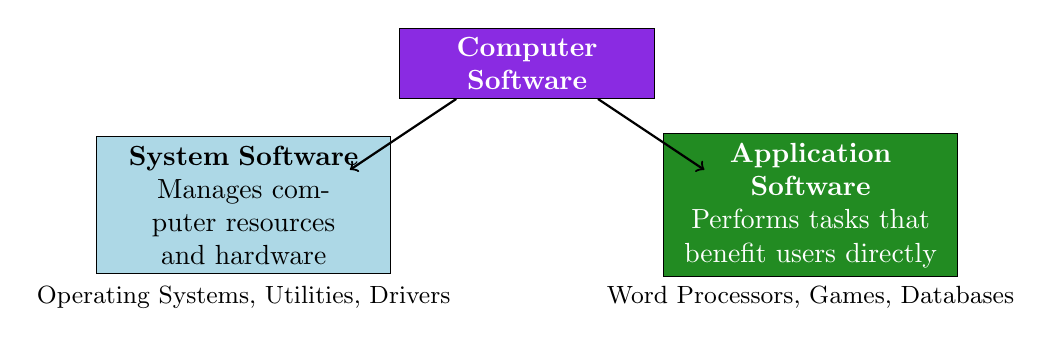
\begin{tikzpicture}[scale=0.9]
            % Main software node
            \node[rectangle, draw, fill=softwareviolet, text=white, text width=3cm, text centered] at (0,2) {\textbf{Computer Software}};
            
            % System software branch
            \node[rectangle, draw, fill=lightblue, text width=3.5cm, text centered] at (-4,0) {\textbf{System Software}\\Manages computer resources\\and hardware};
            
            % Application software branch
            \node[rectangle, draw, fill=evolutiongreen, text=white, text width=3.5cm, text centered] at (4,0) {\textbf{Application Software}\\Performs tasks that\\benefit users directly};
            
            % Arrows
            \draw[->, thick] (-1,1.5) -- (-2.5,0.5);
            \draw[->, thick] (1,1.5) -- (2.5,0.5);
            
            % System software examples
            \node[below] at (-4,-1) {\small{Operating Systems, Utilities, Drivers}};
            
            % Application software examples
            \node[below] at (4,-1) {\small{Word Processors, Games, Databases}};
        \end{tikzpicture}
    \end{center}
    
    \begin{exampleblock}{Hierarchical Relationship}
        System software provides the foundation that enables application software to function effectively.
    \end{exampleblock}
\end{frame}

\begin{frame}{System Software: Foundation Layer}
    \begin{definition}
        System software allows the computer to manage its own resources, control hardware, and provide basic operating functionality.
    \end{definition} 
    
    \textbf{Core Functions:}
    \begin{itemize}
        \item Enables CPU communication with peripherals
        \item Manages keyboard, monitor, printer, scanner, disk drives
        \item Does not solve application or scientific problems
        \item Starts up computer and coordinates all components
    \end{itemize}  
\end{frame}
 

\begin{frame}{System Software: Foundation Layer (cont.)}
   
    \textbf{System Software Components:}
    \begin{columns}
        \begin{column}{0.5\textwidth}
            \begin{itemize}
                \item \textbf{Operating Systems} - Core management
                \item \textbf{Utilities} - Enhancement tools
                \item \textbf{Editors} - Text manipulation
                \item \textbf{Translators} - Language conversion
            \end{itemize}
        \end{column}
        \begin{column}{0.5\textwidth}
            \begin{itemize}
                \item \textbf{Device Drivers} - Hardware interfaces
                \item \textbf{BIOS} - Basic Input/Output System
                \item \textbf{Firmware} - Low-level control
            \end{itemize}
        \end{column}
    \end{columns}
    
    \begin{alertblock}{Critical Role}
        System software is the "mother of all software" - all other software depends on it for operation.
    \end{alertblock}
\end{frame}


\begin{frame}{Operating Systems: The Master Controller}
    \begin{definition}
        The Operating System (OS) acts as the interface between the user and the computer, managing all system resources.
    \end{definition}
    
    \vspace{0.3cm}
    \textbf{Fundamental OS Characteristics:}
    \begin{itemize}
        \item Resides in RAM while computer is ON
        \item Provides resource management services
        \item Cannot operate computer without OS installation
        \item Includes BIOS for resource and internal service management
    \end{itemize}
     
    \textbf{Booting Process:}
    \begin{columns}
        \begin{column}{0.5\textwidth}
         \begin{itemize}
           \item \textbf{Booting Definition:} Process of loading the operating system onto RAM
             
            \item \textbf{Cold Booting:}
            \\Starting computer from completely off state
        \end{itemize}
        \end{column}
        \begin{column}{0.5\textwidth}
        \begin{itemize}
           \item \textbf{Warm Booting:} Restarting computer without turning off power 
           \item  \textbf{System Services:} Time, date, and internal resource management
           \end{itemize}
        \end{column}
    \end{columns}
\end{frame}

\begin{frame}{Operating System Classifications}
    \textbf{OS Types by Application Domain:}
    
    \begin{enumerate}
        \item Real-Time OS
        \begin{itemize}
            \item Special-purpose embedded systems
            \item Applications: robots, cars, modems
            \item Time-critical response requirements
        \end{itemize}
        
        \item Single-user, Single-task OS
        \begin{itemize}
            \item Designed for individual devices
            \item Example: Early mobile phones
            \item One user, one application at a time
        \end{itemize}
        
        \item Single-user, Multitask OS
        \begin{itemize}
            \item Contemporary personal computers
            \item One user, multiple applications
            \item Modern desktop and laptop systems
        \end{itemize}
        
        \item Multi-user OS
        \begin{itemize}
            \item Network environments with shared resources
            \item Server operating systems
            \item Multiple simultaneous users
        \end{itemize}
    \end{enumerate}
\end{frame}

\begin{frame}{Specialized Operating Systems}
    \begin{enumerate}
        \setcounter{enumi}{4}
        \item Network OS
        \begin{itemize}
            \item Resource sharing in network setups
            \item File and printer sharing capabilities
            \item Network administration tools
        \end{itemize}
        
        \item Internet/Web OS
        \begin{itemize}
            \item Browser-based operation
            \item Online functionality focus
            \item Cloud computing integration
        \end{itemize}
        
        \item Mobile OS
        \begin{itemize}
            \item Smartphones, tablets, mobile devices
            \item Touch interface optimization
            \item Power efficiency focus
        \end{itemize}
    \end{enumerate}
    
    % \vspace{0.3cm}
    \textbf{Operating System Examples:}
    \begin{columns}
        \begin{column}{0.3\textwidth}
            \textbf{Desktop OS:}
            \begin{itemize}
                \item Windows 10
                \item Mac OS X
                \item Ubuntu
                % \item Windows XP
            \end{itemize}
        \end{column}
        \begin{column}{0.3\textwidth}
            \textbf{Server OS:}
            \begin{itemize}
                \item Windows Server
                \item Ubuntu Server
                \item Red Hat Enterprise
            \end{itemize}
        \end{column}
        \begin{column}{0.3\textwidth}
            \textbf{Mobile OS:}
            \begin{itemize}
                \item Android OS
                \item iOS
                \item Windows Phone
            \end{itemize}
        \end{column}
    \end{columns}
\end{frame}

\begin{frame}{Operating System Functions}
    \textbf{Core OS Responsibilities:}
    
    \begin{enumerate}
        \item Process Management
        \begin{itemize}
            \item \textbf{Multitasking:} Multiple programs by one user simultaneously
            \item \textbf{Multiprogramming:} Multiple programs on multi-user systems
            \item \textbf{Time-sharing:} Round-robin task processing for multiple users
            \item \textbf{Multiprocessing:} Multiple processors working simultaneously
        \end{itemize}
        
        \item Memory Management
        \begin{itemize}
            \item RAM allocation and deallocation
            \item Virtual memory management
            \item Memory protection between processes
        \end{itemize}
        
        \item Input/Output Handling
        \begin{itemize}
            \item Device communication management
            \item Driver coordination and control
        \end{itemize}
        
        \item Network Communication
        \begin{itemize}
            \item Network protocol management
            \item Resource sharing coordination
        \end{itemize}
    \end{enumerate}
\end{frame}

\begin{frame}{Extended Operating System Functions}
    \begin{enumerate}
        \setcounter{enumi}{4}
        \item File Management
        \begin{itemize}
            \item File system organization and maintenance
            \item Directory structure management
            \item File access permissions and security
        \end{itemize}
        
        \item Security Management
        \begin{itemize}
            \item User authentication and authorization
            \item Data protection and encryption
            \item System access control
        \end{itemize}
        
        \item Device Management
        \begin{itemize}
            \item Hardware detection and installation
            \item Device troubleshooting and maintenance
            \item Plug-and-play functionality
        \end{itemize}
        
        \item System Monitoring
        \begin{itemize}
            \item Performance monitoring through Task Manager
            \item System resource usage tracking
            \item Error detection and reporting
        \end{itemize}
    \end{enumerate}
\end{frame}

\begin{frame}{Utility Programs: System Enhancement Tools}
    \begin{definition}
        Utility programs enhance and expand the functionalities of existing programs, acting as interfaces between system and application software.
    \end{definition}
    
    \vspace{0.3cm}
    \textbf{Essential Utility Categories:}
    
    \begin{enumerate}
        \item Antivirus Software
        \begin{itemize}
            \item Prevents computer virus attacks
            \item Scans hard disks, diskettes, and memory
            \item Examples: Norton, McAfee, AVG, Quickheal, Avast
        \end{itemize}
        
        \item Disk Defragmentation
        \begin{itemize}
            \item Organizes scattered files on drive
            \item Examples: Disk Defragmenter, Perfect Disk, Disk Keeper
        \end{itemize}
        
        \item File Compression
        \begin{itemize}
            \item Optimizes disk space usage
            \item Examples: WinRAR, WinZip, 7-Zip, PeaZip
        \end{itemize}
    \end{enumerate}
\end{frame}

\begin{frame}{Advanced Utility Programs}
    \begin{enumerate}
        \setcounter{enumi}{3}
        \item Data Recovery
        \begin{itemize}
            \item Restores physically damaged or corrupted data
            \item Recovers lost data from various causes
            \item Examples: iCare Data Recovery, Recuva, EaseUs Data Recovery
        \end{itemize}
        
        \item Firewall Protection
        \begin{itemize}
            \item Protection against external threats
            \item Network security management
            \item Example: Windows Firewall, Comodo Free Firewall
        \end{itemize}
    \end{enumerate}
    
    \vspace{0.5cm}
    \textbf{Data Damage Causes:}
    \begin{columns}
        \begin{column}{0.5\textwidth}
            \begin{itemize}
                \item Virus infections
                \item Software malfunctions
                \item Hardware failures
            \end{itemize}
        \end{column}
        \begin{column}{0.5\textwidth}
            \begin{itemize}
                \item Power fluctuations
                \item Human error
                \item System crashes
            \end{itemize}
        \end{column}
    \end{columns}
    
    \begin{alertblock}{Preventive Maintenance}
        Regular use of utility programs helps maintain system health and prevent data loss.
    \end{alertblock}
\end{frame}

\begin{frame}{Device Drivers: Hardware Interfaces}
    \begin{definition}
        Device drivers are system software that enable computer devices and peripherals to function properly by facilitating communication with the operating system.
    \end{definition}
    % \vspace{0.3cm}
    \textbf{Driver Functionality:}
    \begin{itemize}
        \item Enable connected components and peripherals to perform intended tasks
        \item Allow OS to assign duties to hardware devices
        \item Provide interface between hardware and software
        \item Essential for proper device operation
    \end{itemize}
    
    % \vspace{0.3cm}
    \textbf{Devices Requiring Drivers:}
    \begin{columns}
        \begin{column}{0.5\textwidth}
            \begin{itemize}
                \item Mouse - Cursor control
                \item Keyboard - Input interface
                \item Sound card - Audio processing
                \item Display card - Graphics rendering
            \end{itemize}
        \end{column}
        \begin{column}{0.5\textwidth}
            \begin{itemize}
                \item Network card - Connectivity
                \item Printer - Document output
                \item Camera - Image capture
                \item USB devices - Various peripherals
            \end{itemize}
        \end{column}
    \end{columns}
    
    
\end{frame}


\begin{frame}{Device Drivers: Hardware Interfaces(cont.)}
 
   
    \begin{exampleblock}{Default Installation}
        Basic input devices like mouse and keyboard typically have drivers pre-installed with the operating system.
    \end{exampleblock}
\end{frame}

% Section 11: Programming and Translators
\section{Programming Languages and Translators}

\begin{frame}{Translator Systems Overview}
    \begin{definition}
        Translators are system software used for converting programming languages to machine language that computers can understand.
    \end{definition}
     
    \textbf{Common Programming Languages:}
    \begin{columns}
        \begin{column}{0.5\textwidth}
            \begin{itemize}
                \item Python, Java, R, C, C++
                \item FORTRAN (Formula Translation)
                \item PASCAL, BASIC (Beginner's All-purpose Symbolic Instruction Code)
                \item LISP (List Processing)
            \end{itemize}
        \end{column}
        \begin{column}{0.5\textwidth}
             \textbf{Three Types of Translators:}
    \begin{enumerate}
        \item \textbf{Assembler} - Low-level language to machine code
        \item \textbf{Compiler} - High-level language, batch translation
        \item \textbf{Interpreter} - High-level language, line-by-line execution
    \end{enumerate}
        \end{column}
    \end{columns}

    
\end{frame}

\begin{frame}{Detailed Translator Functions}
    \textbf{Assembler:}
    \begin{itemize}
        \item Translates assembly language to machine code
        \item Examples: MASM (Microsoft Assembler), BASM (Borland Assembler), TASM (Turbo Assembler)
        \item Works with low-level programming instructions
    \end{itemize}
    
    % \vspace{0.3cm}
    \textbf{Compiler:}
    \begin{itemize}
        \item Translates \textcolor{blue}{\textbf{entire}}  high-level program at once
        \item Execution occurs after complete translation
        \item Examples: C compiler, Pascal compiler, C++ compiler
        \item Creates executable object files
    \end{itemize}
    
    % \vspace{0.3cm}
    \textbf{Interpreter:}
    \begin{itemize}
        \item Translates and executes programs \textcolor{blue}{\textbf{line by line}}
        \item Immediate execution (step by step)
        \item Examples: Python, MATLAB, Ruby, Perl, PHP, VB6
        \item Interactive programming environment
    \end{itemize}
\end{frame}

\begin{frame}{High-Level Language Categories}
    \textbf{Five Main Types of High-Level Languages:}
    
    \begin{enumerate}
        \item Commercial Languages
        \begin{itemize}
            \item Example: COBOL (Common Business Oriented Language)
            \item Business and administrative applications
        \end{itemize}
        
        \item Scientific Languages
        \begin{itemize}
            \item Example: FORTRAN (Formula Translation)
            \item Mathematical and scientific computing
        \end{itemize}
        
        \item Command Languages
        \begin{itemize}
            \item Examples: C++, SHELL scripts
            \item Operating system interaction
        \end{itemize}
        
        \item Multi-purpose Languages
        \begin{itemize}
            \item Example: BASIC
            \item General-purpose programming applications
        \end{itemize}
    \end{enumerate}
\end{frame}

\begin{frame}{High-Level Language Features}
    \textbf{Key Characteristics:}
    
    \begin{enumerate}
        \item Extensive Vocabulary
        \begin{itemize}
            \item Rich set of words, symbols, and sentences
            \item Human-readable instruction formats
        \end{itemize}
        
        \item Statement Translation
        \begin{itemize}
            \item Programs written in programmer's language
            \item Whole statements translated into multiple machine code instructions
        \end{itemize}
        
        \item Library Integration
        \begin{itemize}
            \item Macros and sub-routines can be incorporated
            \item Reusable code components
        \end{itemize}
        
        \item Machine Independence
        \begin{itemize}
            \item Problem-oriented rather than machine-oriented
            \item Programmers work independently of specific hardware
        \end{itemize}
        
        \item Structured Grammar
        \begin{itemize}
            \item Set of rules must be followed
            \item Similar to written English grammar rules
        \end{itemize}
    \end{enumerate}
\end{frame}

\begin{frame}{Compiler Functions in Detail}
    \textbf{Primary Compiler Responsibilities:}
    
    \begin{enumerate}
        \item Source Code Translation
        \begin{itemize}
            \item Translates source program statements into machine code
            \item Converts human-readable code to executable format
        \end{itemize}
        
        \item Linkage Management
        \begin{itemize}
            \item Includes linkage for closed sub-routines
            \item Connects various program modules
        \end{itemize}
        
        \item Storage Allocation
        \begin{itemize}
            \item Allocates areas of main storage for program execution
            \item Manages memory usage efficiently
        \end{itemize}
        
        \item Object Program Creation
        \begin{itemize}
            \item Produces object program on disk or magnetic tape
            \item Creates executable files for system use
        \end{itemize}
        
        \item Documentation Generation
        \begin{itemize}
            \item Produces printed copy listing of source and object programs
            \item Provides documentation for debugging and maintenance
        \end{itemize}
    \end{enumerate}
\end{frame}

% Section 12: Application Software
\section{Application Software}

\begin{frame}{Application Software Overview}
    \begin{definition}
        Application software performs tasks that directly benefit or assist users in accomplishing specific objectives.
    \end{definition}
    
    % \vspace{0.3cm}
    \textbf{Two Main Categories:}
    
    \begin{columns}
        \begin{column}{0.45\textwidth}
            \begin{block}{Application Packages}
                \textbf{Pre-built software} for specific functions:
                \begin{itemize}
                    \item Not customized but tailored
                    \item Text processing, data analysis
                    \item Statistical analysis, accounting
                    \item Budget analysis applications
                \end{itemize}
            \end{block}
        \end{column}
        \begin{column}{0.45\textwidth}
            \begin{block}{In-house Packages}
                \textbf{Customized software} for specific organizations:
                \begin{itemize}
                    \item Developed by software companies
                    \item Tailored to specific requirements
                    \item Examples: Payroll systems, HR management
                \end{itemize}
            \end{block}
        \end{column}
    \end{columns}
     
\end{frame}


\begin{frame}{Application Software Overview (cont.)}
    
        
    
    \begin{exampleblock}{User-Focused Design}
        Unlike system software, application software is designed with end-user productivity and specific task accomplishment in mind.
    \end{exampleblock}
\end{frame}

\begin{frame}{Word Processing Applications}
    \textbf{Word Processing Packages:}
    
    \begin{columns}
        \begin{column}{0.45\textwidth}
            \textbf{Primary Functions:}
            \begin{itemize}
                \item Processing text documents
                \item Creating memos and letters
                \item Professional document formatting
                \item Editing and revision capabilities
            \end{itemize}
            
            % \vspace{0.3cm}
           
        \end{column}
        \begin{column}{0.55\textwidth}
              \textbf{Popular Examples:}
            \begin{itemize}
                \item \textbf{Microsoft Word} - Industry standard
                \item \textbf{WordStar} - Early word processor
                \item \textbf{AmiPro} - Professional document creation
                \item \textbf{LaTeX} - Scientific document preparation
                \item \textbf{WordPerfect} - Legal and business documents
                \item \textbf{WordPad} - Basic text editing
            \end{itemize}
        \end{column}
    \end{columns}
    
    \begin{alertblock}{Professional Impact}
        Word processing software revolutionized document creation, making professional-quality documents accessible to all users.
    \end{alertblock}
\end{frame}

\begin{frame}{Spreadsheet and Analysis Applications}
    \textbf{Spreadsheet Packages:}
    \begin{itemize}
        \item \textbf{Primary Use:} Data analysis and numerical calculations
        \item \textbf{Examples:} Microsoft Excel, Lotus 1-2-3
        \item \textbf{Capabilities:} Financial modeling, data visualization, statistical analysis
    \end{itemize}
    
    \vspace{0.3cm}
    \textbf{Statistical Packages:}
    \begin{itemize}
        \item \textbf{Purpose:} Advanced statistical analysis and research
        \item \textbf{SPSS:} Statistical Package for Social Scientists
        \item \textbf{SAS:} Statistical Analysis System
        \item \textbf{MINITAB:} Statistical software for quality improvement
        \item \textbf{STATISTICA:} Comprehensive statistical analysis
    \end{itemize}
    
    \vspace{0.3cm}
    \textbf{Accounting Packages:}
    \begin{itemize}
        \item \textbf{Functions:} Accounting and budgeting analysis
        \item \textbf{Examples:} Sage (Line 50, 100, 200, 500), Peachtree, Deacasy
        \item \textbf{Others:} Tally, MS Money, Oracle Financial
    \end{itemize}
\end{frame}

\begin{frame}{Entertainment and Design Applications}
    \textbf{Games Packages:}
    \begin{columns}
        \begin{column}{0.5\textwidth}
            \textbf{Purposes:}
            \begin{itemize}
                \item Relaxation and entertainment
                \item Gaming contests and competitions
                \item Educational gaming
            \end{itemize}
            
            \textbf{Examples:}
            \begin{itemize}
                \item Solitaire, Chess, Scrabble
                \item Monopoly, Super Mario, Awale
                \item Snooker and other sports games
            \end{itemize}
        \end{column}
        \begin{column}{0.5\textwidth}
            % Placeholder for gaming
            % \includegraphics[width=\textwidth]{computer_games.png}
            % \small{\textit{Various computer game interfaces}}
        \end{column}
    \end{columns}
    
    \vspace{0.3cm}
    \textbf{Publishing Packages:}
    \begin{itemize}
        \item \textbf{Purpose:} Graphics design and desktop publishing
        \item \textbf{Examples:} CorelDraw, Microsoft Publisher, Adobe PageMaker
        \item \textbf{Others:} PowerPoint, Paint and other design tools
        \item \textbf{Applications:} Marketing materials, presentations, artwork
    \end{itemize}
\end{frame}

\begin{frame}{Database Management Applications}
    \textbf{Database Management System (DBMS) Packages:}
    
    \begin{columns}
        \begin{column}{0.5\textwidth}
            \textbf{Core Functions:}
            \begin{itemize}
                \item Database design and creation
                \item Data storage and retrieval
                \item Query processing and reporting
                \item Data security and integrity
            \end{itemize}
            
        \end{column}
        \begin{column}{0.5\textwidth}
            % Placeholder for database
            % \includegraphics[width=\textwidth]{database_systems.png}
            % \small{\textit{Database management interface}}
              \textbf{Popular DBMS Examples:}
            \begin{itemize}
                \item \textbf{Microsoft Access} - Desktop database
                \item \textbf{Oracle 8i/9i} - Enterprise database
                \item \textbf{Microsoft SQL Server} - Business database
                \item \textbf{FoxPro} - Database development
                \item \textbf{MySQL} - Open source database
                \item \textbf{Dbase IV} - Early database system
            \end{itemize}
        \end{column}
    \end{columns}
    
    \begin{exampleblock}{Enterprise Integration}
        Modern DBMS applications form the backbone of most business operations, from small businesses to large enterprises.
    \end{exampleblock}
\end{frame}

\begin{frame}{Custom In-House Applications}
    \begin{definition}
        In-house packages are customized software solutions tailored to perform specific functions for particular organizations.
    \end{definition}
    
    \vspace{0.3cm}
    \textbf{Development Process:}
    \begin{itemize}
        \item Created by professional software developers
        \item Designed for specific company requirements
        \item Addresses unique business processes
        \item Provides competitive advantages through customization
    \end{itemize} 
    \textbf{Common In-House Applications:}
    \begin{columns}
        \begin{column}{0.53\textwidth}
            \begin{itemize}
                \item \textbf{Human Resources Management} systems
                \item \textbf{Payroll processing} software
                \item \textbf{Inventory management} systems
                \item \textbf{Customer relationship} management (CRM)
            \end{itemize}
        \end{column}
        \begin{column}{0.47\textwidth}
            \begin{itemize}
                \item \textbf{Manufacturing control} systems
                \item \textbf{Quality assurance} tracking
                \item \textbf{Custom accounting} solutions
                \item \textbf{Enterprise resource planning} (ERP)
            \end{itemize}
        \end{column}
    \end{columns}
    
  
\end{frame}


\begin{frame}{Custom In-House Applications (cont.)}
     
    \begin{alertblock}{Strategic Value}
        Custom in-house software provides organizations with unique capabilities that off-the-shelf solutions cannot match.
    \end{alertblock}
\end{frame}
% Section 13: Computer Functions
\section{Computer Functions Based on Von Neumann Model}

\begin{frame}{Four Essential Computer Operations}
    \textbf{Based on Von Neumann Model Architecture:}
    
    \begin{center}
        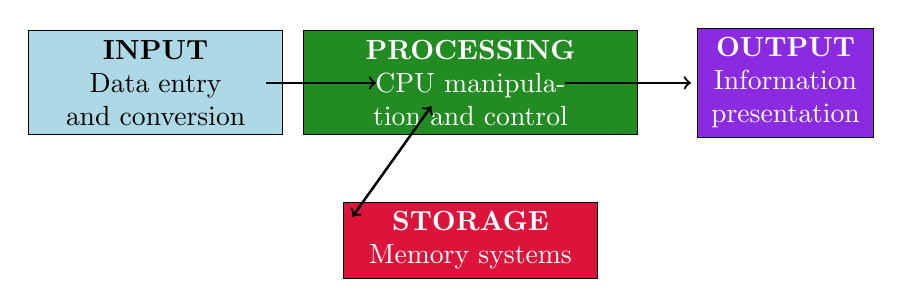
\begin{tikzpicture}[scale=1]
            % Input box
            \node[draw, fill=lightblue, text width=3cm, text centered] at (0,2) {\textbf{INPUT}\\Data entry and conversion};
            
            % Processing box
            \node[draw, fill=evolutiongreen, text=white, text width=4cm, text centered] at (4,2) {\textbf{PROCESSING}\\CPU manipulation and control};
            
            % Storage box
            \node[draw, fill=hardwarered, text=white, text width=3cm, text centered] at (4,0) {\textbf{STORAGE}\\Memory systems};
            
            % Output box
            \node[draw, fill=softwareviolet, text=white, text width=2cm, text centered] at (8,2) {\textbf{OUTPUT}\\Information presentation};
            
            % Arrows showing data flow
            \draw[->, thick] (1.4,2) -- (2.8,2);
            \draw[->, thick] (5.2,2) -- (6.8,2);
            \draw[->, thick] (3.5,1.7) -- (2.5,0.3);
            \draw[->, thick] (2.5,0.3) -- (3.5,1.7);
        \end{tikzpicture}
    \end{center}
    
    \begin{definition}
        For efficient computer operation, these four units must work together seamlessly to process data into meaningful information.
    \end{definition}
\end{frame}

\begin{frame}{INPUT Function: Data Entry System}
    \begin{definition}
        The input function accepts data and converts it into computer-readable form suitable for processing.
    \end{definition}
    
    \vspace{0.3cm}
    \textbf{Input Device Categories:}
    \begin{columns}
        \begin{column}{0.5\textwidth}
            \textbf{Standard Input Devices:}
            \begin{itemize}
                \item Keyboard - Text and command input
                \item Mouse - Pointing and clicking
                \item Microphone - Audio input
                \item Scanner - Document digitization
            \end{itemize}
        \end{column}
        \begin{column}{0.5\textwidth}
            \textbf{Specialized Input:}
            \begin{itemize}
                \item Light pen - Direct screen interaction
                \item Touch screens - Direct manipulation
                \item Barcode readers - Automated data entry
                \item Biometric scanners - Security input
            \end{itemize}
        \end{column}
    \end{columns}
    
    \vspace{0.3cm}
    \begin{exampleblock}{Data Conversion Process}
        Input devices translate human-readable data into binary format (0s and 1s) that computers can process efficiently.
    \end{exampleblock}
\end{frame}

\begin{frame}{PROCESSING Function: The CPU}
    \begin{definition}
        The Central Processing Unit (CPU), also known as the processor, controls and manipulates data to produce information.
    \end{definition}
    
    \vspace{0.3cm}
    \textbf{CPU Architecture:}
    \begin{columns}
        \begin{column}{0.5\textwidth}
            \textbf{Main Components:}
            \begin{itemize}
                \item \textbf{Arithmetic Logic Unit (ALU)}
                \item \textbf{Control Unit (CU)}
                \item \textbf{Registers} - Temporary storage
                \item \textbf{Cache memory} - High-speed access
            \end{itemize}
            
            % \vspace{0.2cm}
           
        \end{column}
        \begin{column}{0.5\textwidth}
             \textbf{Processing Speed:}
            \begin{itemize}
                \item Measured in MHz or GHz
                \item Higher frequency = faster processing
                \item Multiple cores increase performance
            \end{itemize}
        \end{column}
    \end{columns}
    
    \begin{alertblock}{Intel Dominance}
        Intel Corporation processors (8088, 80286, 80386, 80486, Pentium series) are most commonly used in Africa and worldwide.
    \end{alertblock}
\end{frame}

\begin{frame}{CPU Components: ALU and Control Unit}
    \textbf{Arithmetic Logic Unit (ALU):}
    
    \begin{columns}
        \begin{column}{0.5\textwidth}
            \textbf{Arithmetic Operations:}
            \begin{itemize}
                \item \textbf{Addition (A + B)}
                \item \textbf{Subtraction (A - B)}
                \item \textbf{Multiplication (A * B)}
                \item \textbf{Division (A / B)}
            \end{itemize}
            
            % \vspace{0.3cm}
            \textbf{Logical Operations:}
            \begin{itemize}
                \item \textbf{Greater than (A $>$ B)}
                \item \textbf{Equal to (A = B)}
                \item \textbf{Less than (A $<$ B)}
                \item \textbf{Less than or equal (A $<=$ B)}
                \item \textbf{Greater than or equal (A $>=$ B)}
            \end{itemize}
        \end{column}
        \begin{column}{0.5\textwidth}
            \textbf{Control Unit (CU):}
            \begin{itemize}
                \item Coordinates all program instructions
                \item Directs electronic signal movement
                \item Manages communication between:
                \begin{itemize}
                    \item Main memory
                    \item Input devices
                    \item Output devices
                    \item ALU operations
                \end{itemize}
                \item Controls operation speed and timing
            \end{itemize}
             \begin{block}{Motherboard Integration}
        The CPU and supporting components are mounted on the main circuit board called the \textbf{motherboard} or \textbf{system board}.
    \end{block}
        \end{column}
    \end{columns}
    
   
\end{frame}

\begin{frame}{STORAGE Function: Memory Hierarchy}
    \begin{definition}
        Storage provides means for storing data or information temporarily or permanently for future use.
    \end{definition} 
    \vspace{0.3cm}
    \textbf{Two Main Storage Categories:} 
    \begin{columns}
        \begin{column}{0.57\textwidth}
            \begin{block}{Primary Storage}
                \textbf{Main Memory (RAM):}
                \begin{itemize}
                    \item Random Access Memory
                    \item Temporary working space
                    \item Volatile (data lost when power off)
                    \item Holds data and programs for immediate processing
                    \item Mounted on motherboard memory chips
                \end{itemize}
            \end{block}
        \end{column}
        \begin{column}{0.4\textwidth}
            \begin{block}{Secondary Storage}
                \textbf{Permanent Storage:}
                \begin{itemize}
                    \item Non-volatile (retains data without power)
                    \item Easy data retrieval capability
                    \item Examples: Hard disk, CD, flash disk
                    \item Floppy disk, magnetic tape
                \end{itemize}
            \end{block}
        \end{column}
    \end{columns}
   
\end{frame}


\begin{frame}{STORAGE Function: Memory Hierarchy (cont.)} 
    \begin{alertblock}{Memory Capacity Importance}
        Memory capacity determines how large and complex programs can be processed, directly affecting computer performance.
    \end{alertblock}
\end{frame}


\begin{frame}{Secondary Storage Types}
    \textbf{Compact Disk Categories:}

    \begin{columns}
        \begin{column}{0.5\textwidth}

   \begin{enumerate}
        \item[1.] \textbf{CD-ROM Disks}
        \begin{itemize}
            \item Compact Disk Read-Only Memory
            \item Content recorded at manufacture
            \item Cannot be written or erased by user
            \item Example: Music CDs
        \end{itemize}
        
        \item[2.] \textbf{CD-R Disks}
        \begin{itemize}
            \item Compact Disk Recordable
            \item Users can write data once
            \item Can be read by standard CD-ROM drives
            \item Data cannot be changed after recording
        \end{itemize}
        \end{enumerate}
        \end{column}

        \begin{column}{0.5\textwidth} 

         . \begin{enumerate}
              \item[3.] \textbf{CD-RW Disks}
        \begin{itemize}
            \item Compact Disk Re-Writable
            \item Multiple write and erase cycles
            \item Flexible data management
        \end{itemize}
        
        \item[4.] \textbf{DVD/DVD-ROM}
        \begin{itemize}
            \item Digital Versatile Disk
            \item Higher capacity than CDs
            \item Superior video and audio quality
            \item Applications: Movies, games, data storage
        \end{itemize}
    \end{enumerate}

        
        \end{column}

    \end{columns}
 
      
\end{frame}

\begin{frame}{OUTPUT Function: Information Display}
    \begin{definition}
        The output function provides users with means to view information produced by the computer system.
    \end{definition}
    
    % \vspace{0.3cm}
    \textbf{Output Categories:}
    
    \begin{columns}
        \begin{column}{0.5\textwidth}
            \textbf{1. Hard Copy Output: (e.g Printed reports, photos}
            \begin{itemize}
                \item Can be physically held
                \item Paper-based documents 
                \item Permanent physical record
            \end{itemize}
            
            % \vspace{0.3cm}
            \textbf{Output Devices:}
            \begin{itemize}
                \item \textbf{Printers} (inkjet, laser), \textbf{Plotters} for graphics, \textbf{3D printers} for physical objects, etc.
            \end{itemize}
        \end{column}
        \begin{column}{0.5\textwidth}
            \textbf{2. Soft Copy Output (e.g: Screen displays, digital files)}
            \begin{itemize}
                \item Displayed on monitor/screen
                \item Digital format information
                \item Can be saved to storage devices 
            \end{itemize}
            
            % \vspace{0.3cm}
            \textbf{Display Technologies:}
            \begin{itemize}
                \item \textbf{LCD} monitors, \textbf{LED} displays, \textbf{OLED} screens, Projectors, etc.
            \end{itemize}
        \end{column}
    \end{columns}
\end{frame}

% Section 14: Computer Capacity Measurements
\section{Computer Capacity and Measurements}

\begin{frame}{Understanding Digital Storage Units}
    \textbf{Fundamental Storage Measurements:}
    
    \begin{enumerate}
        \item \textbf{Bits (Binary Digits)}
        \begin{itemize}
            \item Smallest unit of data measurement
            \item Binary system values: 0 or 1
            \item Foundation of all computer operations
        \end{itemize}
        
        \item \textbf{Byte}
        \begin{itemize}
            \item Standard unit for computer data
            \item Equal to 8 bits
            \item Represents one character
        \end{itemize}
        
        \item \textbf{Kilobyte (KB)}
        \begin{itemize}
            \item Approximately 1,000 bytes
            \item Actually 1,024 bytes (2\^{10})
            \item Rounded for practical use
        \end{itemize}
        
        \item \textbf{Megabyte (MB)}
        \begin{itemize}
            \item About 1 million bytes
            \item Actually 1,024 × 1,024 = 1,048,576 bytes
            \item Rounded to 1,000,000 bytes
        \end{itemize}
    \end{enumerate}
\end{frame}

\begin{frame}{Large Scale Storage Measurements}
    \begin{enumerate}
        \setcounter{enumi}{4}
        \item \textbf{Gigabyte (GB)}
        \begin{itemize}
            \item About 1 billion bytes
            \item Actually 1,024³ = 1,073,741,824 bytes
            \item Rounded to 1,000,000,000 bytes
            \item Common unit for hard disk capacity
        \end{itemize}
        
        \item \textbf{Terabyte (TB)}
        \begin{itemize}
            \item About 1 trillion bytes
            \item 1,009,511,627,776 bytes exactly
            \item Used for supercomputer main memory
            \item Modern large storage systems
        \end{itemize}
    \end{enumerate}  
\end{frame}

\begin{frame}{Large Scale Storage Measurements (cont.)} 
    \begin{center}
        \textbf{Conversion Hierarchy:}
        \\
        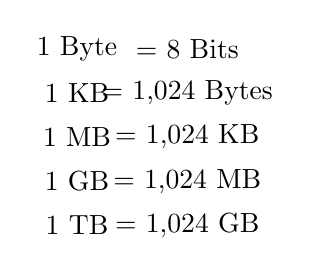
\begin{tikzpicture}[scale=0.7]
            \node at (0,0) {1 Byte};
            \node at (2,0) {= 8 Bits};
            
            \node at (0,-0.8) {1 KB};
            \node at (2,-0.8) {= 1,024 Bytes};
            
            \node at (0,-1.6) {1 MB};
            \node at (2,-1.6) {= 1,024 KB};
            
            \node at (0,-2.4) {1 GB};
            \node at (2,-2.4) {= 1,024 MB};
            
            \node at (0,-3.2) {1 TB};
            \node at (2,-3.2) {= 1,024 GB};
        \end{tikzpicture}
    \end{center}
\end{frame}
\begin{frame}{Practical Conversion Examples}
    \textbf{Step-by-Step Conversion Problems:}
    
    \textbf{Example 1: Convert 4 bytes to bits}
    \begin{itemize}
        \item 1 byte = 8 bits
        \item 4 bytes = 4 × 8 bits = \textbf{32 bits}
    \end{itemize}
    
    \vspace{0.1cm}
    \textbf{Example 2: Convert 5 KB to bytes}
    \begin{itemize}
        \item 1 KB = 1,024 bytes
        \item 5 KB = 5 × 1,024 bytes = \textbf{5,120 bytes}
    \end{itemize}
    
    \vspace{0.1cm}
    \textbf{Example 3: Convert 12 MB to KB}
    \begin{itemize}
        \item 1 MB = 1,024 KB
        \item 12 MB = 12 × 1,024 KB = \textbf{12,288 KB}
    \end{itemize}
    
    \vspace{0.1cm}
    \begin{exampleblock}{Complex Conversion}
        \textbf{Convert 4MB5KB to bits:}
        \\4MB = 4,194,304 bytes, 5KB = 5,120 bytes
        \\Total = 4,199,424 bytes = 33,595,392 bits
    \end{exampleblock}
\end{frame}

% Section 15: Computer Classification by Size
\section{Computer Classification by Size}

\begin{frame}{Computer Size Categories}
    \textbf{Four Main Computer Classes:}
    
    \begin{enumerate}
        \item[1.] \textbf{Supercomputers}
        \begin{itemize}
            \item Fastest and highest-capacity computers
            \item Most expensive systems available
            \item Applications: Weather forecasting, oil exploration
            \item Aircraft design, mathematical research
            \item Hundreds to thousands of processors
        \end{itemize}
        
        \item[2.] \textbf{Mainframe Computers}
        \begin{itemize}
            \item Only computers available until late 1960s
            \item Less powerful than supercomputers but still fast
            \item Mid to large size, large capacity machines
            \item Multiple processors for enhanced performance
        \end{itemize}
        
        \item[3.] \textbf{Minicomputers}
        \begin{itemize}
            \item Small computers with portability features
            \item Tower units, desktops, laptops, palmtops
            \item Stand-alone or network-connected usage
            \item Local Area Network (LAN) capabilities
        \end{itemize}
    \end{enumerate}
\end{frame}

\begin{frame}{
Computer Size Categories (Cont.)}
    % \textbf{Microcomputers (Personal Computers):}
    \begin{enumerate}
        \item[4.] \textbf{Microcomputers: Personal Computing}

\begin{columns}
        \begin{column}{0.45\textwidth}
            \textbf{Historical Development:}
            \begin{itemize}
                \item Introduced in early 1980s
                \item Less expensive than larger systems
                \item Easier installation compared to mainframes/supercomputers
                \item Designed for individual users
            \end{itemize}
            
            % \vspace{0.3cm}
            
        \end{column}
        \begin{column}{0.45\textwidth}
            % Placeholder for microcomputer types
            % \includegraphics[width=\textwidth]{microcomputer_types.png}
            % \small{\textit{Various microcomputer form factors}}
            \textbf{Microcomputer Types:}
            \begin{itemize}
                \item \textbf{Desktop/PC} - Standard office computer
                \item \textbf{Laptop} - Portable computing
                \item \textbf{Notebook} - Ultra-portable design
                \item \textbf{Palmtop} - Handheld devices
                \item \textbf{Programmable Calculator} - Specialized computing
            \end{itemize}
        \end{column}
    \end{columns}
        
    \end{enumerate} 
    \begin{alertblock}{Personal Computing Revolution}
        Microcomputers democratized computing power, making advanced computational capabilities available to individuals and small organizations.
    \end{alertblock}
\end{frame}

% Section 16: Computer Types
\section{Computer Types: Digital, Analog, and Hybrid}

\begin{frame}{Three Computer Types by Processing Method}
    \textbf{Classification by Data Representation:}
    
    \begin{enumerate}
        \item \textbf{Digital Computers}
        \begin{itemize}
            \item Data represented in discrete/discontinuous form
            \item Based on ON/OFF or two-state conditions
            \item Uses binary number system (0 and 1)
            
            \item Most common type in modern computing
            \item \textbf{Examples:} Digital wristwatch, desktop PC
        \end{itemize}
        
        \item \textbf{Analog Computers}
        \begin{itemize}
            \item Data represented in continuous form
            \item Physical measurement applications
            
            \item Used for real-time physical monitoring
            \item \textbf{Examples:} Thermometer, barometer
        \end{itemize}
        
        \item \textbf{Hybrid Computers}
        \begin{itemize}
            \item Combines features of both analog and digital
            \item Best of both processing methods
            \item Used in specialized applications
        \end{itemize}
    \end{enumerate}
\end{frame}

\begin{frame}{Digital vs Analog Signal Representation}
    \begin{columns}
        \begin{column}{0.5\textwidth}
            \textbf{Digital Signal Characteristics:}
            \begin{itemize}
                \item Discrete, step-like representation
                \item Clear distinction between states
                \item Binary values: 0 and 1
                \item High noise resistance
                \item Precise data representation
            \end{itemize} 
            
            \begin{center}
                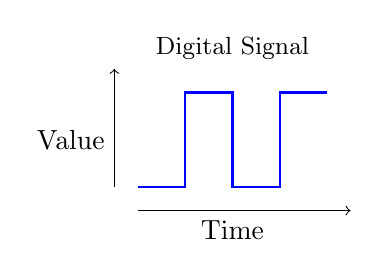
\begin{tikzpicture}[scale=0.6]
                    % Digital signal representation
                    \draw[thick, blue] (0,0) -- (1,0) -- (1,2) -- (2,2) -- (2,0) -- (3,0) -- (3,2) -- (4,2);
                    \draw[->] (0,-0.5) -- (4.5,-0.5);
                    \draw[->] (-0.5,0) -- (-0.5,2.5);
                    \node[below] at (2,-0.5) {Time};
                    \node[left] at (-0.5,1) {Value};
                    \node[above] at (2,2.5) {\small{Digital Signal}};
                \end{tikzpicture}
            \end{center}
        \end{column}
        \begin{column}{0.5\textwidth}
            \textbf{Analog Signal Characteristics:}
            \begin{itemize}
                \item Continuous, smooth representation
                \item Infinite possible values
                \item Natural physical phenomena
                \item Susceptible to noise
                \item Real-world measurements
            \end{itemize}
            
            \begin{center}
                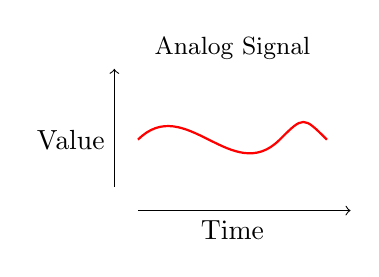
\begin{tikzpicture}[scale=0.6]
                    % Analog signal representation
                    \draw[thick, red] (0,1) .. controls (1,2) and (2,0) .. (3,1) .. controls (3.5,1.5) .. (4,1);
                    \draw[->] (0,-0.5) -- (4.5,-0.5);
                    \draw[->] (-0.5,0) -- (-0.5,2.5);
                    \node[below] at (2,-0.5) {Time};
                    \node[left] at (-0.5,1) {Value};
                    \node[above] at (2,2.5) {\small{Analog Signal}};
                \end{tikzpicture}
            \end{center}
        \end{column}
    \end{columns}
    
\end{frame}


\begin{frame}{Digital vs Analog Signal Representation} 
    \begin{exampleblock}{Application Domains}
        Digital computers dominate general computing, while analog computers excel in real-time measurement and control systems.
    \end{exampleblock}
\end{frame}

% Section 17: Input and Output Devices
\section{Input and Output Devices}

\begin{frame}{Input Devices: Data Entry Systems}
    \begin{definition}
        Input devices translate data into a form the computer can process, enabling human-computer interaction.
    \end{definition} 
    % \vspace{0.3cm}
    \textbf{Primary Input Devices:}
    
    \begin{columns}
        \begin{column}{0.45\textwidth}
            \textbf{Standard Input:}
            \begin{itemize}
                \item \textbf{Keyboard} - Text and command entry
                \item \textbf{Mouse} - Pointing and selection
                \item \textbf{Joystick} - Gaming and control
                \item \textbf{Touchpad} - Laptop navigation
                \item \textbf{Trackball} - Precision pointing
            \end{itemize}
        \end{column}
        \begin{column}{0.55\textwidth}
            \textbf{Specialized Input:}
            \begin{itemize}
                \item \textbf{MICR} - Magnetic Ink Character Recognition
                \item \textbf{OCR} - Optical Character Recognition
                \item \textbf{OMR} - Optical Mark Recognition
                \item \textbf{Scanner} - Document digitization
                \item \textbf{Barcode Reader} - Automated identification
            \end{itemize}
        \end{column}
    \end{columns}
    
    \begin{alertblock}{Evolution Trend}
        Modern input devices are becoming more intuitive, supporting voice, touch, and gesture-based interactions.
    \end{alertblock}
\end{frame}

\begin{frame}{Detailed Keyboard Layout and Functions}
    \textbf{Keyboard Components (5 Main Sections):}

    \begin{columns}
        \begin{column}{0.45\textwidth}
              \begin{enumerate}
        \item[1.] \textbf{Function Keys (F1-F12)}
        \begin{itemize}
            \item Programmable function keys
            \item Application-specific shortcuts
            \item System command access
        \end{itemize}
        
        \item[2.] \textbf{Control Keys}
        \begin{itemize}
            \item Insert, Delete, Home, End
            \item Page Up, Page Down, Pause
            \item Print Screen, Scroll Lock
        \end{itemize}

\item[3.] \textbf{Alphanumeric Keys}
        \begin{itemize}
            \item Letters A-Z, numbers 0-9
            \item Spacebar (longest key)
            \item Backspace, Enter, Shift, Ctrl, Alt
            \item Tab, Caps Lock, special characters
        \end{itemize}
        \end{enumerate}

        \end{column}

        \begin{column}{0.6\textwidth}
         \begin{enumerate}
                 
        
        \item[4.] \textbf{Arrow/Cursor-Movement Keys}
        \begin{itemize}
            \item Four directional arrows
            \item Move cursor around screen text
            \item Navigation in documents and interfaces
        \end{itemize}

        \item[5.] \textbf{Numeric Keypad}
        \begin{itemize}
            \item Dual-purpose functionality
            \item \textbf{Num Lock ON:} Calculator-style number input (1,2,3...9)
            \item \textbf{Num Lock OFF:} Arrow keys and navigation (Page Up/Down)
        \end{itemize}
  \end{enumerate}
        \end{column}

\end{columns}


        
 
        
    
  
\end{frame}

\begin{frame}{Keyboard Functions Continued}
    % \begin{enumerate}
    %     \setcounter{enumi}{4}
    %     \item \textbf{Numeric Keypad}
    %     \begin{itemize}
    %         \item Dual-purpose functionality
    %         \item \textbf{Num Lock ON:} Calculator-style number input (1,2,3...9)
    %         \item \textbf{Num Lock OFF:} Arrow keys and navigation (Page Up/Down)
    %     \end{itemize}
    % \end{enumerate}
    
    % \vspace{0.5cm}
    \textbf{Cursor Control:}
    \begin{itemize}
        \item \textbf{Cursor (Insertion Point):} Shows where data will be entered next
        \item \textbf{Arrow Key Functions:}
        \begin{itemize}
            \item Move cursor right
            \item Move cursor left  
            \item Move cursor up
            \item Move cursor down
        \end{itemize}
    \end{itemize}
    
    \begin{exampleblock}{Professional Usage}
        Understanding keyboard layout and shortcuts significantly improves productivity in professional computing environments.
    \end{exampleblock}
\end{frame}

\begin{frame}{Mouse and Pointing Devices}
    \textbf{Mouse Functionality:}
    
    \begin{columns}
        \begin{column}{0.5\textwidth}
            \textbf{Basic Components:}
            \begin{itemize}
                \item Left button (primary)
                \item Right button (secondary/context)
                \item Scroll wheel (modern mice)
                \item Mouse pad for optimal tracking
            \end{itemize}
            
        \end{column}
        \begin{column}{0.5\textwidth}
              \textbf{Mouse Operations:}
            \begin{itemize}
                \item \textbf{Point:} Position cursor
                \item \textbf{Click:} Select items
                \item \textbf{Double-click:} Execute programs
                \item \textbf{Drag:} Move objects
                \item \textbf{Right-click:} Context menus
            \end{itemize} 
        \end{column}
    \end{columns}
    
       \begin{block}{Pointer Display}
        The mouse pointer symbol on screen indicates the current position and enables precise interaction with graphical interfaces.
    \end{block}
\end{frame}



\begin{frame}{Mouse and Pointing Devices (cont.)}
     \textbf{Alternative Pointing Devices:}
    
    \begin{columns}
        \begin{column}{0.5\textwidth} 

 \textbf{1. Joystick:}
            \begin{itemize}
                \item Primarily for video/TV games
                \item Pointing and control device
                \item Gaming and simulation applications
            \end{itemize}
            
        \end{column}
        \begin{column}{0.5\textwidth}
        
            \textbf{2. Trackball:}
            \begin{itemize}
                \item Same function as mouse
                \item Moveable ball on stationary device
                \item Rotated with fingers
                \item Like an upside-down mouse
            \end{itemize}
        \end{column}
    \end{columns}
    
  
\end{frame}

\begin{frame}{Specialized Recognition Systems}
    \textbf{Advanced Input Recognition Technologies:}
    
    \begin{enumerate}
        \item \textbf{MICR (Magnetic Ink Character Recognition)}
        \begin{itemize}
            \item Printed with magnetized ink
            \item Read by MICR equipment producing digitized signals
            \item Bank reader/sorter machines for check processing
            \item Financial transaction automation
        \end{itemize}
        
        \item \textbf{OCR (Optical Character Recognition)}
        \begin{itemize}
            \item Reads special OCR character sets (OCR fonts)
            \item Converts text to machine-readable form
            \item Applications: Utility bills, price tags, glasses prescriptions
            \item Examples: Water Corporation bills, NEPA bills
        \end{itemize}
        
        \item \textbf{OMR (Optical Mark Recognition)}
        \begin{itemize}
            \item Reads pencil marks and converts to computer-usable form
            \item Famous applications: SAT, GRE examinations
            \item Multiple-choice test processing
            \item Survey and assessment automation
        \end{itemize}
    \end{enumerate}
\end{frame}

\begin{frame}{Document Scanning Technology}
    \textbf{Scanner Functionality:} 
    \begin{columns}
        \begin{column}{0.5\textwidth}
            \textbf{Primary Functions:}
            \begin{itemize}
                \item Scanning text documents
                \item Image digitization and processing
                \item Document archival and storage
                \item Integration with computer processing
            \end{itemize}
            
            % \vspace{0.3cm}
            
        \end{column}
        \begin{column}{0.5\textwidth}
        \textbf{Scanning Technologies Include:}
            \begin{itemize}
                \item Barcode readers for retail
                \item MICR for banking applications
                \item OCR for text recognition
                \item OMR for form processing
            \end{itemize}
            % Placeholder for scanner types
            % \includegraphics[width=\textwidth]{scanner_types.png}
            % \small{\textit{Various scanner technologies}}
        \end{column}
    \end{columns}
    
    \begin{exampleblock}{Document Management}
        Scanners enable conversion of physical documents to digital format, facilitating storage, retrieval, and processing.
    \end{exampleblock}
\end{frame}

\begin{frame}{Output Devices: Information Presentation}
    \begin{definition}
        Output devices serve as interfaces between users and computers, presenting information in soft or hard copy formats.
    \end{definition}
    
    \vspace{0.3cm}
    \textbf{Major Output Device Categories:}
    
    \begin{columns}
        \begin{column}{0.5\textwidth}
            \textbf{Printers:}
            \begin{itemize}
                \item Print characters, symbols, graphics on paper
                \item Two main types: Impact and Non-impact
            \end{itemize}
             
            \textbf{Impact Printers:}
            \begin{itemize}
                \item Physical contact with paper
                \item Examples: Dot matrix, line printer
                \item Mechanical printing mechanism
            \end{itemize}
             
        \end{column}
        \begin{column}{0.5\textwidth} 
            \textbf{Monitors:}
            \begin{itemize}
                \item TV-like devices for display
                \item Show instructions, messages, data
                \item Various sizes: 14 to 21+ inches
                \item Different technologies and resolutions
            \end{itemize}
        \end{column}
    \end{columns}
\end{frame}



\begin{frame}{Output Devices: Information Presentation (cont.)}
     
    \textbf{Major Output Device Categories:}
    
    \begin{columns}
        \begin{column}{0.5\textwidth}  
            \textbf{Non-impact Printers:}
            \begin{itemize}
                \item No physical contact with paper
                \item Examples: Laser jet, desk jet
                \item Higher quality, quieter operation
            \end{itemize}
        \end{column}
        \begin{column}{0.5\textwidth}
            \textbf{Plotters:}
            \begin{itemize}
                \item Specialized high-quality graphics output
                \item Variety of colors available
                \item Two common types: Flatbed and Drum
                \item Engineering and design applications
            \end{itemize} 
             
        \end{column}
    \end{columns}
\end{frame}


\begin{frame}{Monitor Types and Technologies}
    \textbf{Display Technology Categories:}
    
    \begin{enumerate}
        \item \textbf{Monochrome Monitors}
        \begin{itemize}
            \item Display only one color on background
            \item Usually black text on white background
            \item Becoming obsolete in modern computing
            \item Still found in some specialized applications
        \end{itemize}
        
        \item \textbf{Color Monitors (RGB)}
        \begin{itemize}
            \item Red, Green, Blue color system
            \item Display 16 colors to 16.7 million colors
            \item Color depth/bit depth determines range
            \item Most software developed for color displays
        \end{itemize}
    \end{enumerate}
    
    \vspace{0.5cm}
    \begin{exampleblock}{RGB Technology}
        RGB (Red, Green, Blue) monitors create all visible colors by combining these three primary light colors in different intensities.
    \end{exampleblock}
\end{frame}

\begin{frame}{Monitor Resolution Standards}
    \textbf{Display Resolution Categories:}
    
    \begin{enumerate}
        \item \textbf{VGA (Video Graphics Array/Adapter)}
        \begin{itemize}
            \item Supports 16 to 256 colors
            \item Resolution dependent on color depth:
            \item 320×200 pixels: 256 colors
            \item 640×480 pixels: 16 colors (4-bit color)
        \end{itemize}
        
        \item \textbf{SVGA (Super Video Graphics Array/Adapter)}
        \begin{itemize}
            \item Supports 256 colors at higher resolution
            \item Graphics modes: 800×600 and 1024×768 pixels
            \item Called 8-bit color depth
            \item Better quality than standard VGA
        \end{itemize}
        
        \item \textbf{XGA/EGA (Extended Graphics Array/Adapter)}
        \begin{itemize}
            \item High-resolution display capability
            \item Supports up to 16.7 million colors
            \item 1024×768 pixels resolution
            \item 24-bit color or "true color"
            \item Memory chip dependent performance
        \end{itemize}
    \end{enumerate}
\end{frame}

% Section 18: Activities and Assessment
\section{Learning Activities and Assessment}

\begin{frame}{Learning Activities and Questions}
    \textbf{Historical and Technical Questions:}
    
    \begin{enumerate}
        \item When was the word "Computer" first used?
        \item Which is the first commercial computer?
        \item When and who invented the first computer mouse?
        \item Who is the father of the computer?
        \item When was the first keyboard invented?
        \item What operating system do we use in the computer lab?
        \item How have computers affected your life as a student?
        \item List the four functions of an operating system.
    \end{enumerate}
    
    \vspace{0.5cm}
    \textbf{Comparative Analysis:}
    \begin{enumerate}
        \item Differentiate between mainframe and microcomputer
        \item Why is microcomputer referred to as PC?
        \item Can small and large computers perform the same tasks? Discuss.
    \end{enumerate}
\end{frame}

\begin{frame}{Practical Conversion Exercises}
    \textbf{Storage Capacity Conversions:}
    
    \begin{enumerate}
        \item Convert 15MB to TB
        \item Convert 20TB to KB  
        \item Convert 8MB to Bits
        \item Convert 4 bytes to bits
        \item Convert 5 KB to bytes
        \item Convert 12MB to KB
    \end{enumerate}
    
    \vspace{0.5cm}
    \textbf{Sample Solution Process:}
    \begin{exampleblock}{Example: Convert 4 bytes to bits}
        \textbf{Given:} 1 byte = 8 bits
        \\
        \textbf{Solution:} 4 bytes = 4 × 8 bits = 32 bits
    \end{exampleblock}
    
    \begin{alertblock}{Study Tip}
        Master the conversion hierarchy: Bit → Byte → KB → MB → GB → TB, with each level being 1,024 times larger (except bit to byte = 8).
    \end{alertblock}
\end{frame}

% Section 19: Unit Summary
\section{Comprehensive Unit Summary}

\begin{frame}{Unit 3 Achievement Summary}
    \textbf{Knowledge Areas Mastered:}
    
    \begin{columns}
        \begin{column}{0.5\textwidth}
            \textbf{Historical Understanding:}
            \begin{itemize}
                \item Computer evolution from Pascal to modern systems
                \item Five generations of computer development
                \item Key historical figures and contributions
                \item Technological progression patterns
            \end{itemize}
            
            \vspace{0.3cm}
            \textbf{Technical Knowledge:}
            \begin{itemize}
                \item Hardware and software relationships
                \item Operating system functions
                \item Input/output device operations
                \item Storage capacity measurements
            \end{itemize}
        \end{column}
        \begin{column}{0.5\textwidth}
            \textbf{Practical Applications:}
            \begin{itemize}
                \item Computer usage in various sectors
                \item Personal computer selection criteria
                \item Understanding side effects and benefits
                \item Computer classification systems
            \end{itemize}
            
            \vspace{0.3cm}
            \textbf{System Understanding:}
            \begin{itemize}
                \item Von Neumann model application
                \item System vs application software
                \item Digital vs analog processing
                \item Computer size categories
            \end{itemize}
        \end{column}
    \end{columns}
\end{frame}

\begin{frame}{Key Concepts Integration}
    \textbf{Interconnected Learning Themes:}
    
    \begin{enumerate}
        \item \textbf{Evolution Pattern:} Consistent improvement in size, cost, reliability, and performance across generations
        
        \item \textbf{System Integration:} Hardware and software work together; neither can function independently
        
        \item \textbf{User-Centric Design:} Modern computers focus on user experience and accessibility
        
        \item \textbf{Application Versatility:} Computers adapt to countless industries and use cases
        
        \item \textbf{Technological Convergence:} Multiple technologies combine to create comprehensive computing solutions
    \end{enumerate}
    
    \vspace{0.5cm}
    \begin{alertblock}{Foundation Complete}
        This unit provides the essential historical, technical, and practical foundation needed for advanced computer science studies.
    \end{alertblock}
\end{frame}

 

\begin{frame}{Final Thoughts and Discussion}
    \begin{center}
        \Large{\textbf{The Computing Journey Continues}}
    \end{center}
     
    \textbf{Key Takeaways:}
    \begin{itemize}
        \item Computers have transformed from room-sized machines to portable devices
        \item Each generation brought revolutionary improvements in capability and accessibility
        \item Understanding both benefits and limitations helps us use technology effectively
        \item The foundation principles remain consistent despite rapid technological change
    \end{itemize} 
    \begin{center}
        \textbf{Questions, Discussion, and Clarifications}
    \end{center}
\end{frame}

\end{document}